\epigraph{\textit{The most damaging phrase in the English language is "we have always done it this way".}}{-- \textup{Grace Hopper}}

We have examined two distinct Scala and Apache Spark-based solutions up to this point. Both were, as we have mentioned, far from ideal. We have to start from scratch if we want to find a more sophisticated solution.

\section{Technology stack}

\begin{figure}[ht]
    \centering
    \newsavebox\mybox
    \savebox{\mybox}{\includegraphics[width=.3\linewidth]{img/9-1_rust.jpg}}
    \begin{subfigure}{.3\textwidth}
        \centering
        \usebox{\mybox}
        \caption{Rust programming language}
    \end{subfigure}%
    \hspace*{0.1em}
    \begin{subfigure}{.3\textwidth}
        \centering
        \vbox to \ht\mybox{%
            \vfill
            \includegraphics[width=.9\linewidth]{img/9-2_duckdb.png}
            \vfill
        }
        \caption{DuckDB}
    \end{subfigure}%
    \hspace*{0.1em}
    \begin{subfigure}{.3\textwidth}
        \centering
        \vbox to \ht\mybox{%
            \vfill
            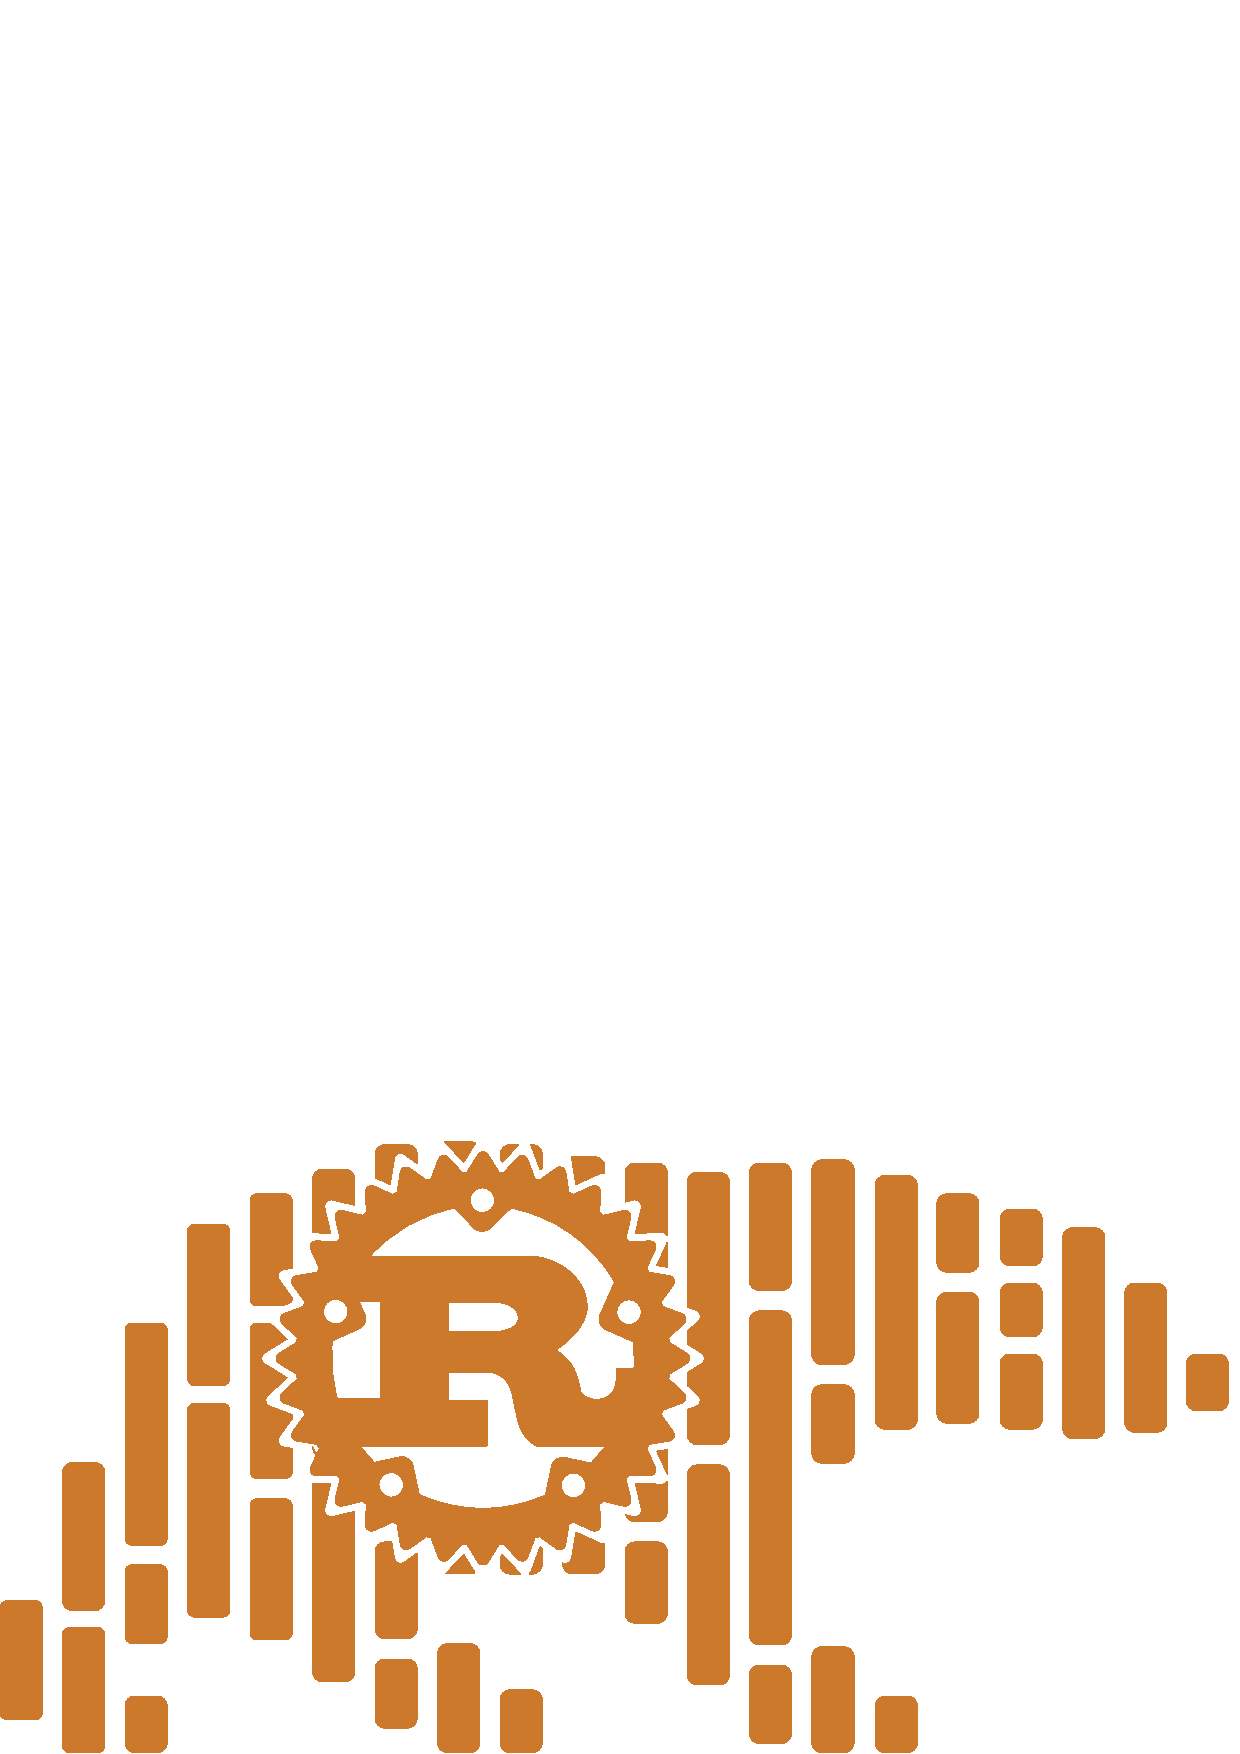
\includegraphics[width=.8\linewidth]{img/9-3_polars.pdf}
            \vfill
        }
        \caption{Pola-rs}
    \end{subfigure}%
    \caption{Stack of the different technologies we are using for the third solution}
\end{figure}

\subsection{Rust}

Rust is a multi-purpose, high-level programming language. Its primary focus is on performance, memory safety, and concurrency. In this perspective, Rust might be considered a modern language; as of March 18th, 2023, the most recent stable release is version 1.68. For achieving memory safety and concurrency, both at the same time, Rust prevents data races through a \textit{borrow checker} that tracks the object and allows each memory position to have only one owner at a time. Rust is popular for systems programming, and was included by the Linux kernel in December 2022, but it also has some high-level functional constructs like pattern-matching and the neatly implemented \texttt{Enums}.

The key features of Rust are:

\begin{enumerate}
    \itemsep0.5em
    \item \textbf{Performance:} It accomplishes this by employing a static memory management strategy rather than a garbage collector, using ownership instead. This means that the compiler decides when memory is allocated and released at compile time. Rust can produce incredibly effective code as a result.
    \item \textbf{Memory safety:} Rust is designed to be memory safe. It achieves this by using a borrow checker. This means that the compiler determines at compile time when memory is accessed, allowing Rust to prevent memory issues like use-after-free and double-free.
    \item \textbf{Concurrency:} Rust is designed to be concurrent. This means that Rust programs can be executed in partial order, or out-of-order, without affecting the outcome. This allows the parallel execution of the concurrent units, significantly increasing the performance of the program in multi-threaded systems.
\end{enumerate}

An example of a simple \textit{Hello World} program written in Rust is shown below.

\begin{code}[Hello World written in Rust]
    \inputminted{rust}{code/listings/9-1_helloWorld.rs}
\end{code}

\subsection{DuckDB}

Conversely, DuckDB is a C++-based in-process SQL OLAP database management system that is intended to be integrated into other applications. This means that DuckDB follows the ACID model and supports popular SQL constructs like window functions, table expressions, and JSON. Additionally, it is column-oriented and created with analytical queries in mind. The impact of this last remark on the scope of our project will be explained further below. Being a project that is only a few years old, DuckDB is still being actively developed.

The key features of DuckDB are:

\begin{enumerate}
    \itemsep0.5em
    \item \textbf{In-process:} DuckDB is an embedded database that runs in the same process as the application. This means that there is no separate server process that needs to be started, stopped, or configured. The application can directly interface with DuckDB through a C API.
    \item \textbf{OLAP or On-Line Analytical Processing:} DuckDB is designed for OLAP workloads. It is optimized for analytical queries that scan large amounts of data and perform complex aggregations.
    \item \textbf{Columnar:} DuckDB is a columnar database. This means that data is stored in columns instead of rows. This can dramatically minimize the amount of data that needs to be read from memory because DuckDB can now only read the columns needed for a query. The vectorized query execution method, which enables incredibly quick query execution, benefits from the column orientation as well. Last but not least, the compression efficiency of the columnar storage format can help to further reduce the quantity of data that needs to be read from memory.
\end{enumerate}

\subsection{Pola-rs}

Pola-rs is a fast and memory-efficient DataFrame library for Rust. It is built on Apache Arrow, a cross-language development platform for in-memory data. This means that data can be shared between languages without the need for serialization or deserialization. Many well-known data science and analytics frameworks, such as Apache Parquet, Apache Spark, Dask, and Polars, employ Apache Arrow. Putting it all together, Pola-rs is a DataFrame implementation written in Rust, a data structure that is commonly used in data science and analytics.

The key features of Pola-rs are:

\begin{enumerate}
    \itemsep0.5em
    \item \textbf{Zero-copy:} Pola-rs is a DataFrame library that uses Apache Arrow as the memory model. This means that Polars does not copy data when performing operations on the DataFrame. Instead, it manipulates the metadata of the underlying Arrow array. This makes Polars very fast and memory efficient.
    \item \textbf{Parallel execution:} Pola-rs is designed to be parallel. This means that Polars can execute operations on multiple threads at the same time. This allows Pola-rs to take advantage of multi-core systems, resulting in faster execution.
    \item \textbf{Lazy evaluation:} Pola-rs is designed to be lazy. This means that Polars does not execute operations until they are needed. This allows Pola-rs to avoid unnecessary computations, resulting in faster execution.
    \item \textbf{Query optimization:} Pola-rs' Lazy API optimizes the query plan for it to be executed faster. This means that Polars can optimize queries by reordering operations and removing unnecessary operations. This allows queries to be executed faster.
    \item \textbf{Streaming:} Pola-rs is designed to allow streams from external files. This means that Polars can process data in batches read from an external file or database. This allows Pola-rs to process data without having to load it all into memory first, resulting in faster execution.
\end{enumerate}

\section{Extract-Transform-Load}

The Extract-Transform-Load (ETL) process is a data integration method aiming at extracting data from one or more sources, transforming it, and loading the result into a target system. An ETL process is a critical component of data-intensive applications, as having properly structured and valid data has a strong impact on the quality of the results and the performance of the system. With that said, the ETL process is used in data migration projects, where data is moved from one system to another. This last remark is important because it is the case of our project, where we are willing to move data from a JSON file to a relational database.

\subsection{Extract}

The first step of the ETL process is the extraction of data from the source system. This step is responsible for connecting to the source system and retrieving the data. The source system can be a database, a file, or even a web service.

\subsection{Transform}

The second step of the ETL process is the transformation of data. This step is responsible for converting the data from its source format to the target format. This step is also responsible for cleaning the data, removing duplicates, and performing other operations to ensure that the data is valid and consistent. In our case, we want to transform the data from a JSON format to DuckDB. Not only that, but we also have to store the data in a way that is consistent with the knowledge graph model. This means that we have to extract the entities and relationships from the data and represent them in a graph format. See section \ref{section:wd2duckdb_design} for more details.

\subsection{Load}

The third and final step of the ETL process is the loading of data into the target system. This step is responsible for connecting to the target system and inserting the data.

For us to accomplish what we have just described, we will need to use a tool that can perform the ETL process. In our case, we will implement one ourselves using Rust. This tool will be responsible for extracting data from a JSON file, transforming it into a relational format, and loading it into a DuckDB database. The tool will be called \texttt{wd2duckdb}. See chapter \ref{chapter:wd2duckdb} for more details.

\section{Knowledge Graph Subsets}

Having our data in a relational database is not enough. We have to implement a system for us to query the knowledge graph in a Pregel fashion. This system will be called \texttt{pregel-rs}. What's more, an algorithm for the creation of the subsets is also needed. This algorithm will be called \texttt{pschema-rs}. See chapter \ref{chapter:pschema} for more details.